%================================================================== Logo On/Off
\LogoOff

%==================================================================FRONT PAGE AND TOC
% For article only
\mode<presentation:0>{\thispagestyle{empty}\maketitle}

% For presentation only
\mode<presentation| article:0| handout:0>{
    \begin{frame}<article:0>[label=portada]
    \titlepage
    \end{frame}%Fin del frame
}

% For handout only
\mode<handout>{
  \begin{frame}[label=portada]
    \maketitle
  \end{frame}
}

%% TABLE OF CONTENTS
\begin{frame}[label=toc]
    \mode<article:0>{\frametitle{Contents}}
    \mode<presentation>{\small}
    \tableofcontents%[hidesubsections]
\end{frame}

%%%==================================================================S INTRODUCTION
\section{\textquestiondown Qué es el LiDAR aéreo?}
%%%==================================================================Sb
%\subsection{Principios}
%%%==================================================================F 
%\begin{frame}
%    \frametitle{Principios del LiDAR aéreo}
%    \begin{enumerate}
%        \item El LiDAR aéreo (Airborne Laser Scanner, \alert<1>{ALS}) es la combinación de:
%	\uncover<1->{
%	\begin{itemize}
%	 \item \alert<1,2>{Escaner Laser}
%	 \item \alert<1,3>{GPS}, que nos da la posición del sensor.
%	 \item \alert<1,3>{IMU}, que nos da nuestra orientación del avión.
%	\end{itemize}
%	}
%	\uncover<2->{
%	\item La posición con respecto al sensor de un punto en tierra se determina por:
%	\begin{itemize}
%	 \item El \alert<2>{tiempo} que tarda cada impulso desde que es emitido hasta que es recibido.
%	 \item El \alert<2>{ángulo} medido desde el nadir en el cual ha sido emitido el rayo.
%	\end{itemize}
%	}
%	\uncover<3>{\item  La posición relativa combinada con la posición global (\alert<3>{GPS}) y la orientación (\alert<3>{IMU}) nos permiten calcular las coordenadas (X,Y,Z) en el punto medido en tierra en un sistema de posicionamiento global (WGS84)}
%    \end{enumerate}
%\end{frame}
%%%==================================================================Sb
%\subsection{Características}
%%%==================================================================F
%\begin{frame}[label=lidar_charact]
%    \frametitle{Características del ALS}
%    \begin{enumerate}[<+->]
%    	\item \alert<1>{Alta precisión} tanto en la componente planimétrica como en la altrimétrica
%    	\item \alert<2>{Alta resolución} debido a la frecuencia de medición.
%    	\item \alert<3>{Monoscópica} y casi \alert{nadiral} $\Rightarrow$ permite observar el terreno incluso en zonas de gran vegetación
%    \end{enumerate}
%\end{frame}
%%==================================================================Sb
\subsection{Primer y último impulso}
%%==================================================================F 
\mode<beamer>{
  \pgfdeclareimage[height=40mm]{roof}{images/roof}
  \pgfdeclareimage[height=40mm]{tree}{images/tree}
}
\mode<beamer:0>{
  \pgfdeclareimage[height=40mm]{roofg}{images/roof_grey}
  \pgfdeclareimage[height=40mm]{treeg}{images/tree_grey}
}
\begin{frame}[label=firstlast1]
    \frametitle{Primer y último impulso}
    \begin{enumerate}[<+->]
        \item Debido a la divergencia del láser, pueden recibirse \alert<1>{más de un eco} para el mismo rayo.
	\item Los sensores actuales son capaces de medir al menos dos retornos: \alert<2>{primero} y \alert<2>{último}
	\item Normalmente se producen por: \alert<3->{bordes} de edificios \uncover<4->{o \alert<4>{vegetación}}
    \end{enumerate}
    \begin{center}
   	\begin{tikzpicture}
	\mode<beamer>{
    	  \uncover<3->{\pgftext[bottom,left,at={\pgfpointxy{-2}{0}}]{\pgfuseimage{roof}}}
    	  \uncover<4>{\pgftext[bottom,left,at={\pgfpointxy{2}{0}}]{\pgfuseimage{tree}}}
	}
	\mode<beamer:0>{
    	  \pgftext[bottom,left,at={\pgfpointxy{-2}{0}}]{\pgfuseimage{roofg}}
    	  \pgftext[bottom,left,at={\pgfpointxy{2}{0}}]{\pgfuseimage{treeg}}
	}
	\end{tikzpicture}
    \end{center}
\end{frame}
%%==================================================================F 
\begin{frame}
    \frametitle{\textquestiondown Para qué sirve?}
    \begin{enumerate}[<+->]
     \item Una diferencia considerable entre el primer y último impulso puede ser una pista para detectar vegetación y otros objetos: edificios, puentes, tendidos eléctricos...
     \item Los últimos impulsos tienen más probabilidad de ser terreno.
     \item Mediante una simple interpolación:
     	\begin{itemize}
     	   \item Primer impulso: creación de Modelo Digital de Superficie (\alert<4>{MDS})
     	   \item \'Ultimo impulso: ``creación'' de Modelo Digital del Terreno (\alert<5>{MDT})
     	\end{itemize}
     \item Hay pocas posibilidades de, sin hacer ningún análisis, distinguir entre un punto \alert<6>{objeto} y uno \alert<6>{terreno}.
    \end{enumerate}
\end{frame}
%%==================================================================S
\section{Filtros ALS}
%%==================================================================Sb
\subsection{Definición}
%%==================================================================F
\begin{frame}[label=filter_def]
    \frametitle{Filtros ALS}
    \onslide<1->\begin{beamerboxesrounded}[shadow=true]{Definición: \emph{Nube de puntos LiDAR}}
     Es un conjunto de puntos tridimensionales con un atributo asociado: $V = \left\lbrace v=\left(x,a\right) | x \in \mathbb{R}^3, a \in \mathbb{N} \right\rbrace$
    \end{beamerboxesrounded}

    \onslide<2->{Clasificación la nube de puntos como:
    \begin{itemize}
 	\item 1, si el punto pertenece a un \alert<2>{objeto}
 	\item<3-> 0, si el punto pertenece al \alert<3>{terreno}
    \end{itemize}}

    \onslide<4>\begin{beamerboxesrounded}[shadow=true]{Definición: \emph{Filtrar}}
     Consiste en \alert<4>{eliminar} los puntos de $V$ con atributo igual 1 (objeto) y dejar los clasificados como 0 (terreno).
    \end{beamerboxesrounded}
\end{frame}
%%==================================================================Sb
\subsection{Tipos de filtros/clasificaciones}
%%==================================================================F
\begin{frame}
    \frametitle{Tipos de clasificaciones}
    \begin{itemize}
        \item Morfológicos
        \item Cluster
        \item Segmentación
        \item ....
        \item Estudio de pendientes (splines)
    \end{itemize}
\end{frame}
%%==================================================================Sc
\section{Clasificación mediante splines}
%%==================================================================Sb
\begin{frame}
  \frametitle{Objetivos y metodología}
  \begin{enumerate}[<+->]
    \item Objetivo:
    \begin{itemize}
       \item Generar un MDT, un modelo de vegetación, un modelo de edificios...
    \end{itemize}
    \item ¿Cómo?:
    \begin{itemize}
 	\item Clasificando puntos en diferentes categorías: terreno, objeto y
            vegetación.
        \item Interpolación de superficies mediante un ajuste de mínimos
            cuadrados de splines utilizando una norma de Tychonov
    \end{itemize}
  \end{enumerate}
\end{frame}
%%==================================================================Sb
\subsection{Splines}
%%==================================================================F
\begin{frame}
    \frametitle{Spline bilineares y bicúbicas}
    \begin{center}
        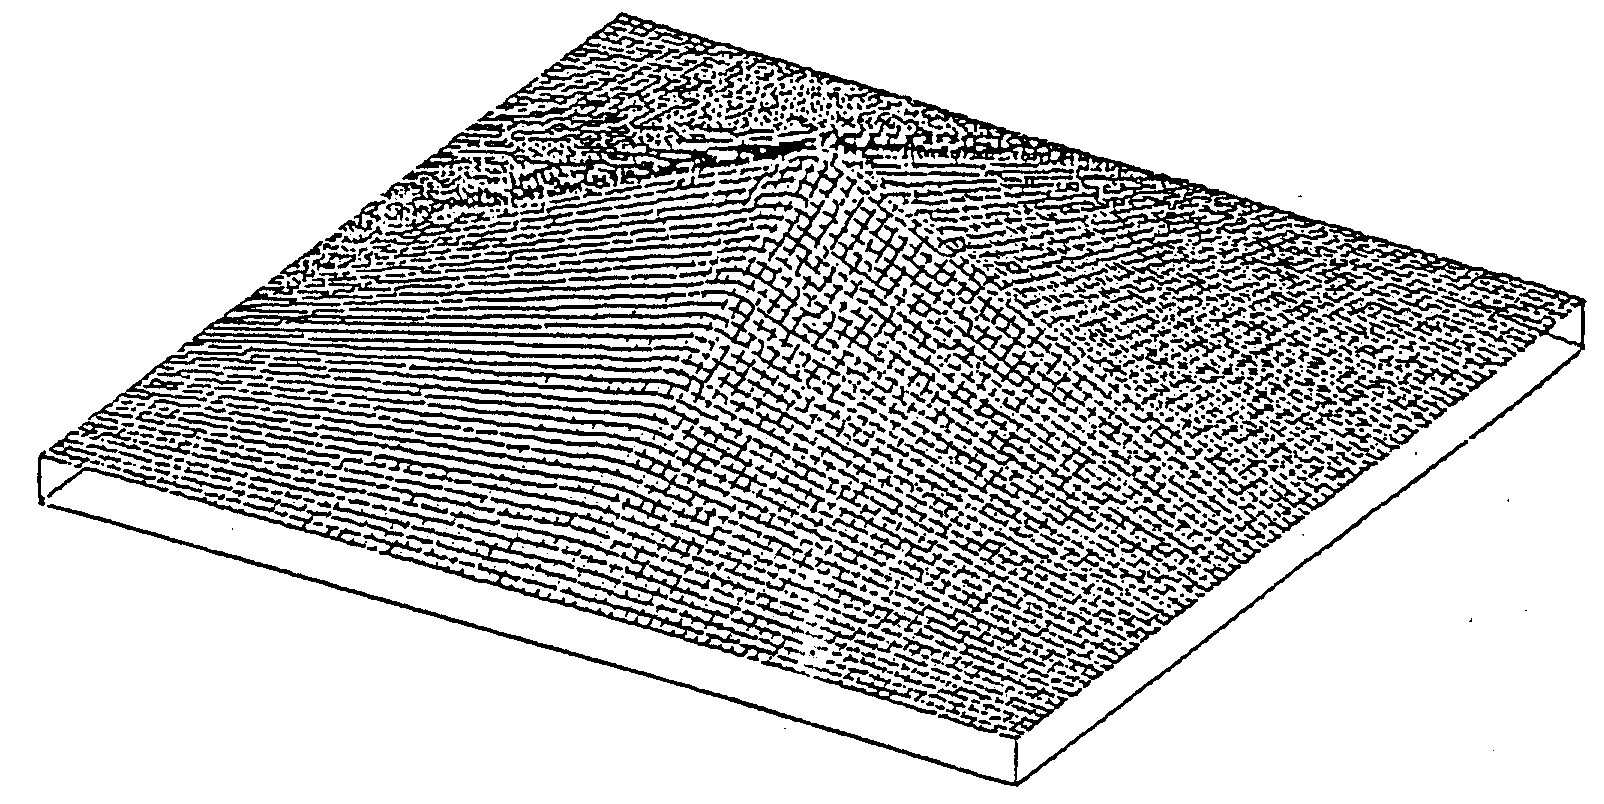
\includegraphics[width=0.45\textwidth]{images/bilinear_spline.jpg}
        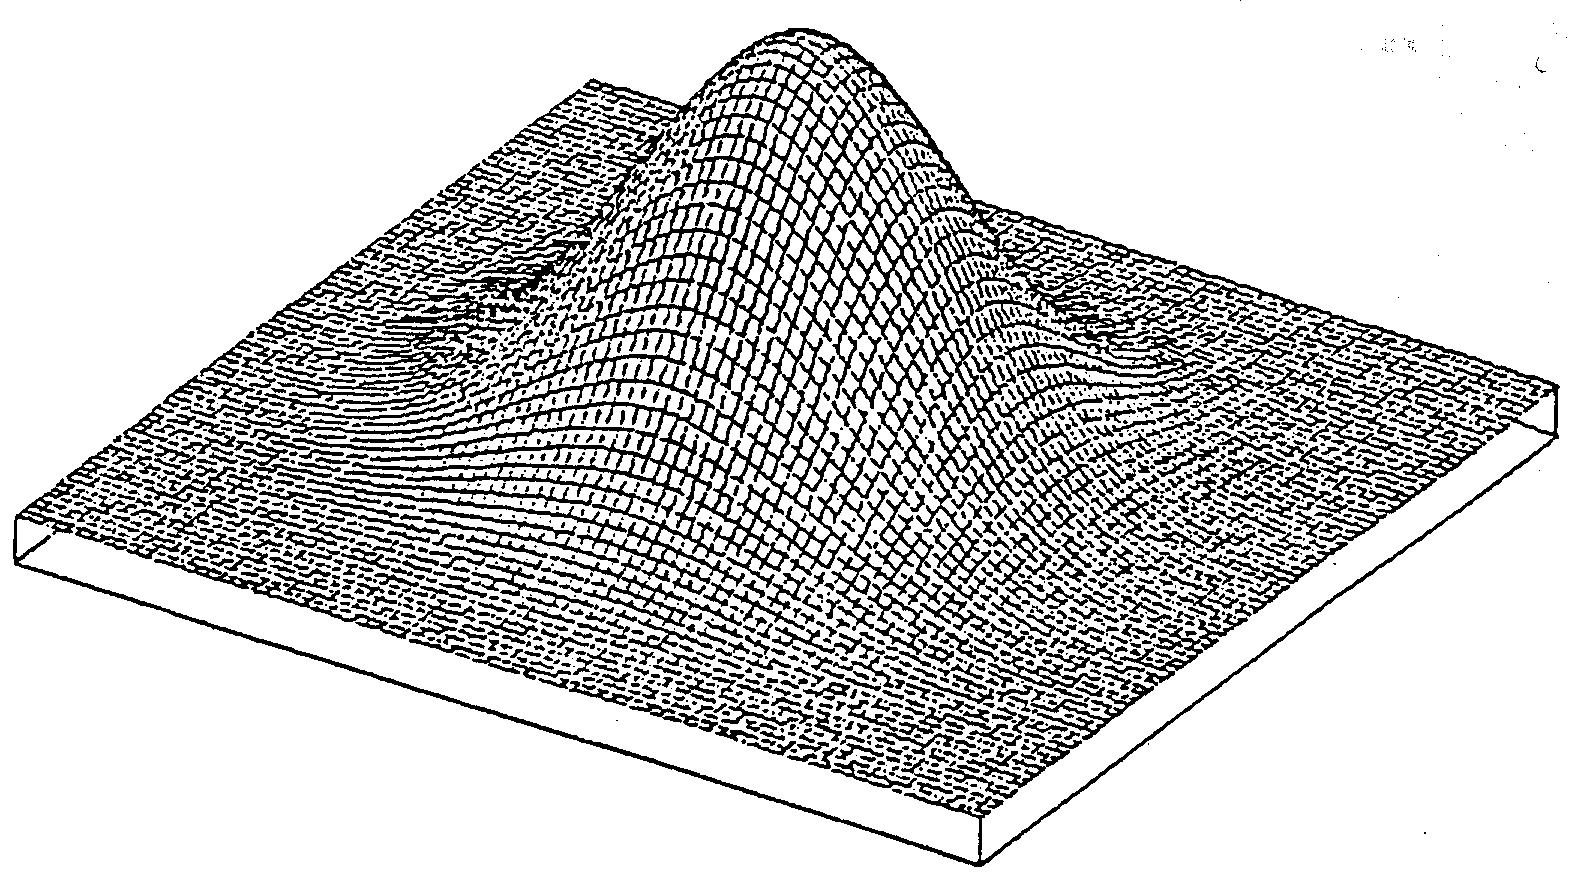
\includegraphics[width=0.45\textwidth]{images/bicubic_spline.jpg}
        %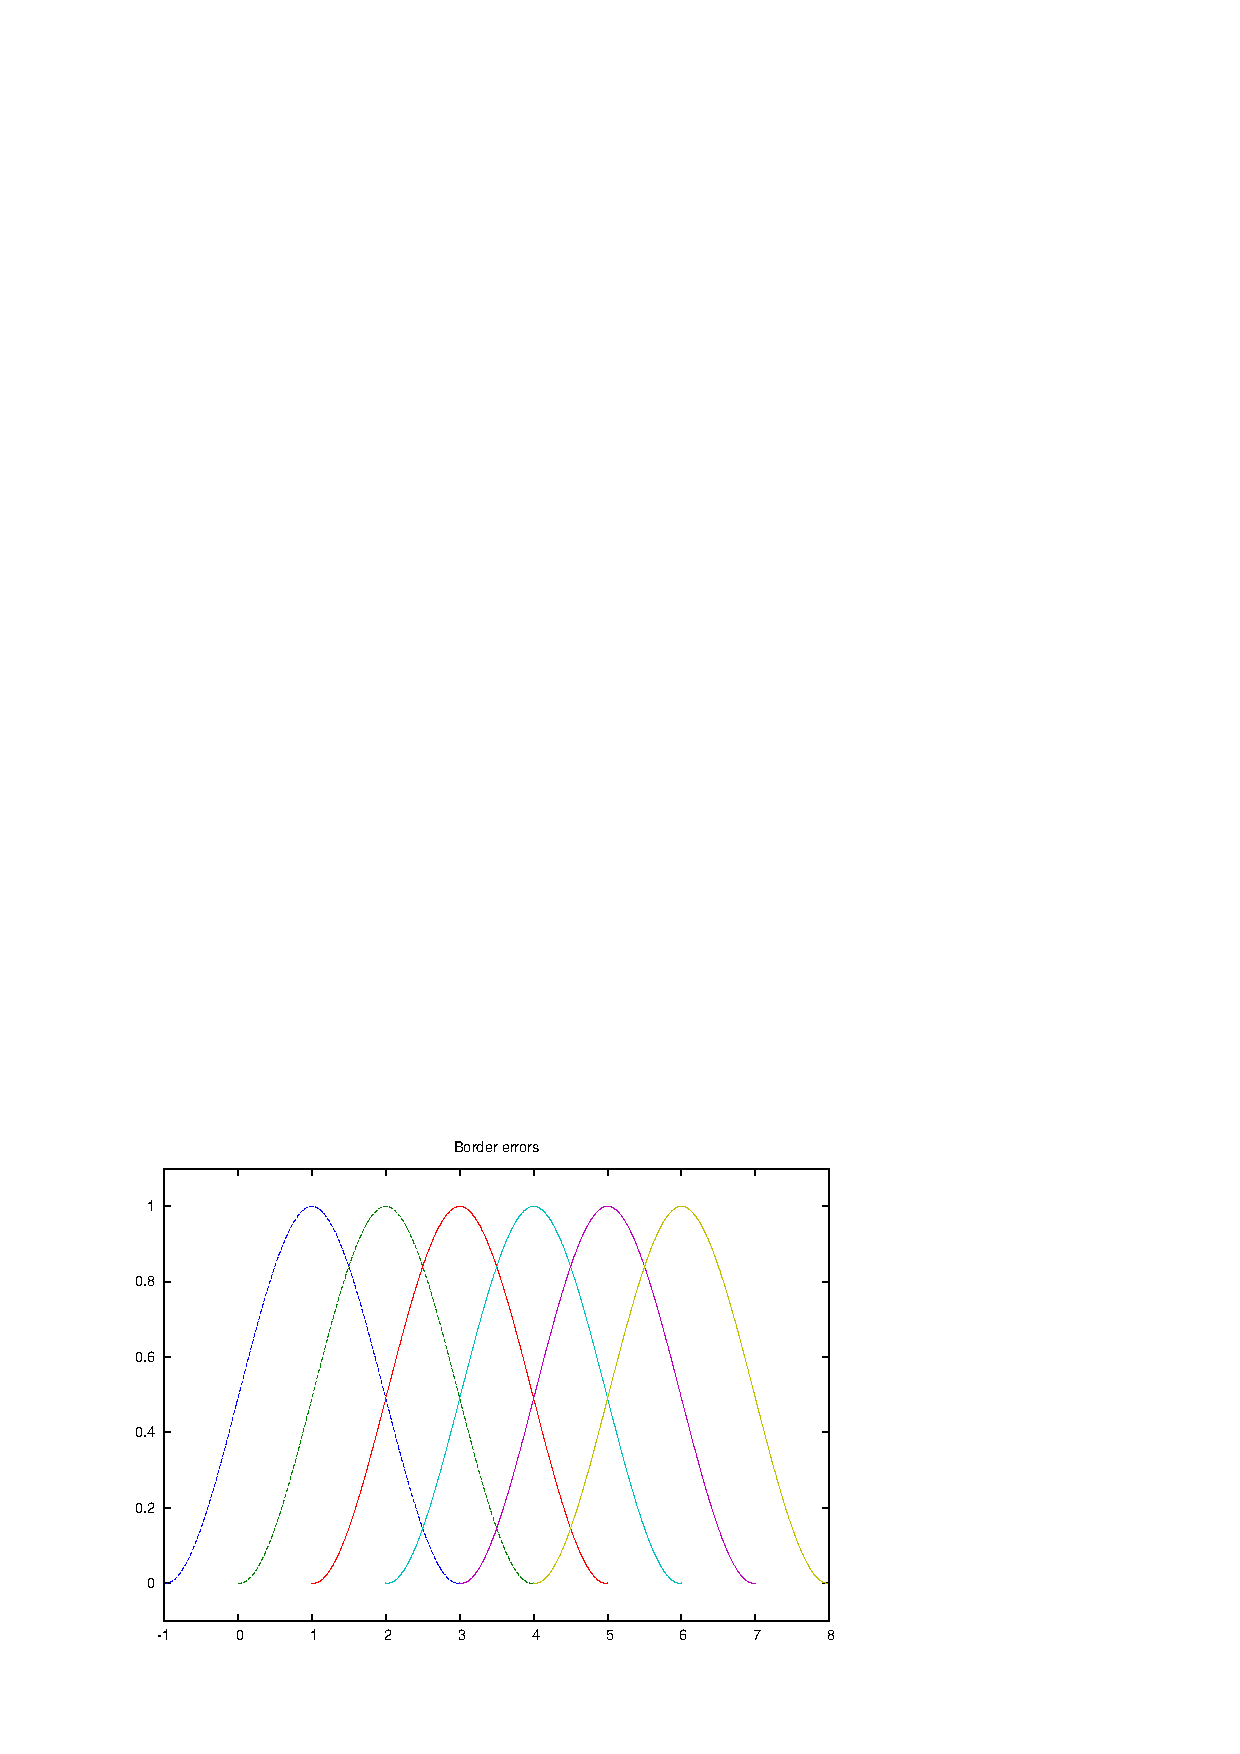
\includegraphics[width=0.45\textwidth]{images/border_errors.jpg}
    \end{center}
\end{frame}
%%==================================================================Sb
\subsection{Puntos groseros}
%%==================================================================F
\begin{frame}
   \frametitle{Puntos groseros}
   \begin{enumerate}
    \item Hay siempre puntos anómalos debido a diferentes eventos:
     \begin{itemize}
 	\item<2-> \alert<2,3,6>{Pájaros}
 	\item<4-> \alert<4,6>{Nubes de agua}
 	\item<5-> \alert<5,6>{``Multipath''}...
     \end{itemize}
    \item<6>{\alert<6>{\textexclamdown\textexclamdown Deben ser eliminados!!}} 
   \end{enumerate}
   \begin{picture}(0,100)
       \uncover<2>{\put(10,10){
\includegraphics[height=30mm]{images/angry_birds}}}     
       \uncover<3,6>{\put(10,10){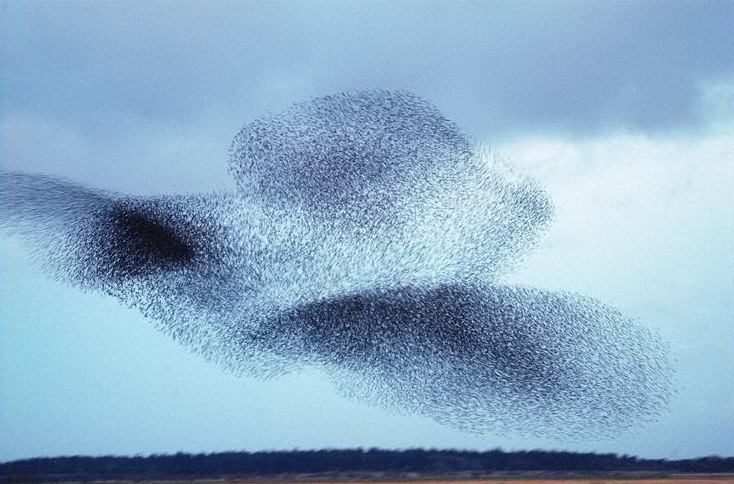
\includegraphics[height=30mm]{images/bandada}}}
       \uncover<4>{\put(50,10){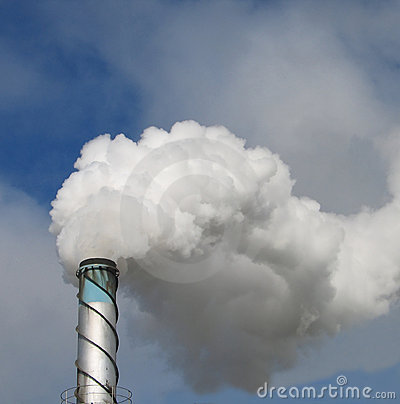
\includegraphics[height=30mm]{images/vapor_chimenea}}}
       \uncover<4,6>{\put(150,10){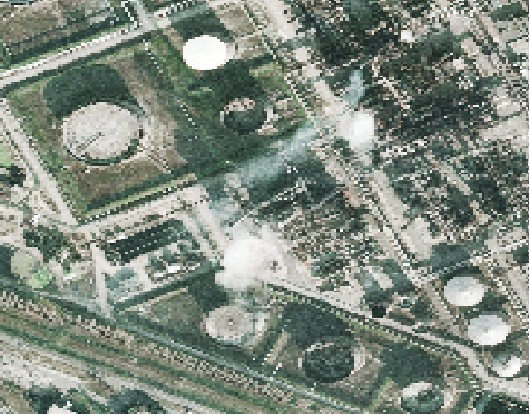
\includegraphics[height=30mm]{images/fumo}}}
       \uncover<5,6>{\put(280,10){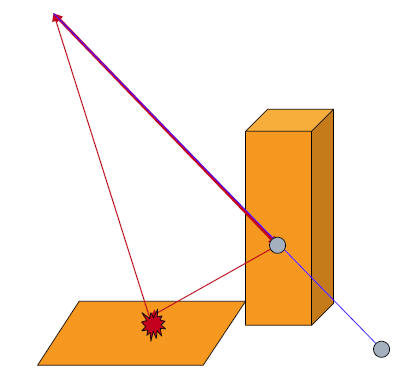
\includegraphics[height=30mm]{images/multipath}}}
    \end{picture}
\end{frame}
%%==================================================================F
\begin{frame}
   \frametitle{Detección de puntos groseros}
   \begin{itemize}
    \item<1-> La eliminación se hace mediante una interpolacion con splines 
        bicúbicas bastante lisa y baja resolución.
    \item<8-> Aquellos puntos que se alejen más de un umbral determinado son 
        considerados como puntos groseros y eliminados.
    \item<9-> El umbral por defecto son \alert<8>{$50~m$}
   \end{itemize}

    \begin{picture}(0,100)
       \only<2>{\put(80,0){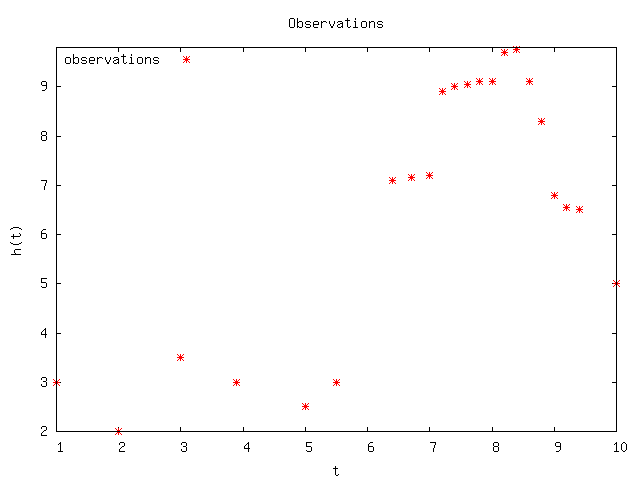
\includegraphics[height=35mm]{images/obs_splines}}}
       \only<3,8->{\put(80,0){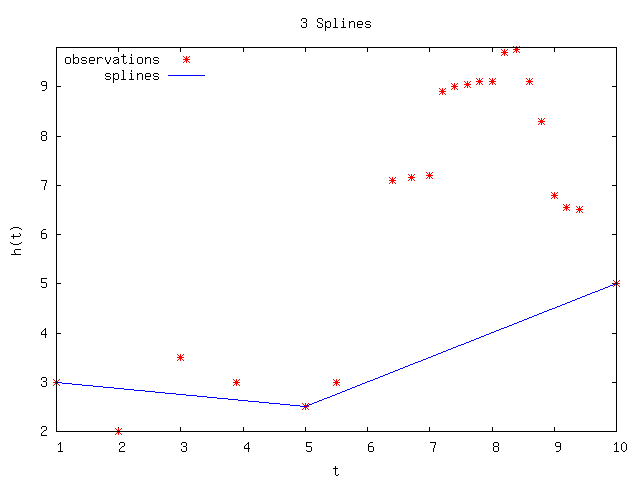
\includegraphics[height=35mm]{images/3splines}}}
       \only<4>{\put(80,0){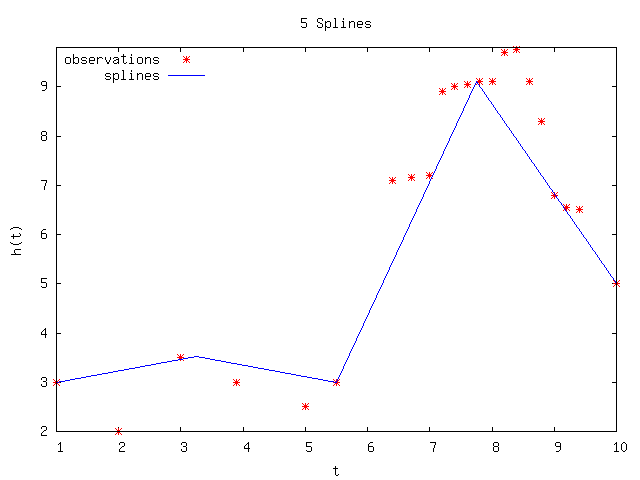
\includegraphics[height=35mm]{images/5splines}}}
       \only<5>{\put(80,0){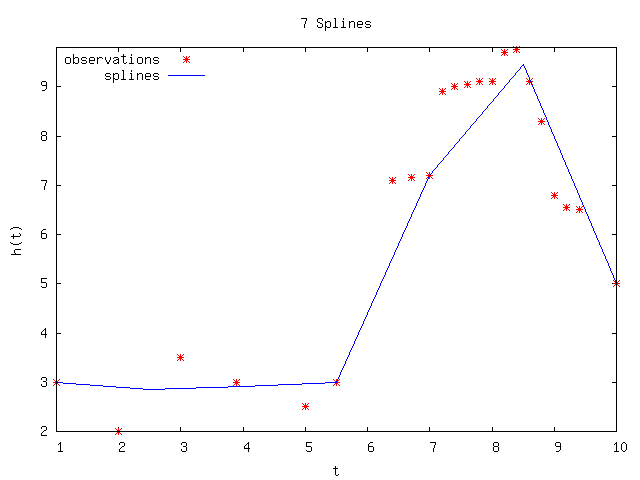
\includegraphics[height=35mm]{images/7splines}}}
       \only<6>{\put(80,0){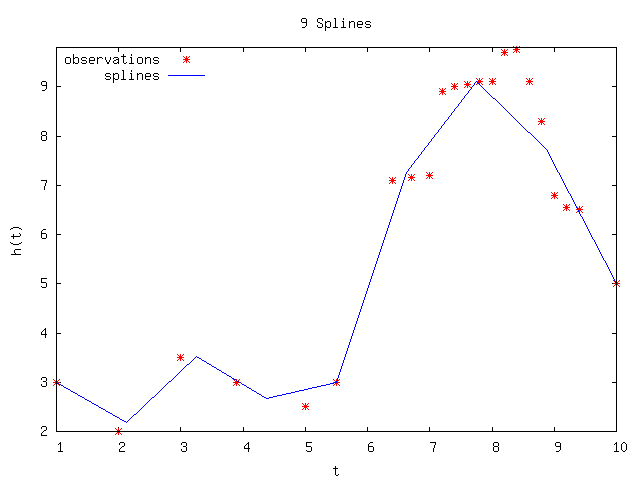
\includegraphics[height=35mm]{images/9splines}}}
       \only<7>{\put(80,0){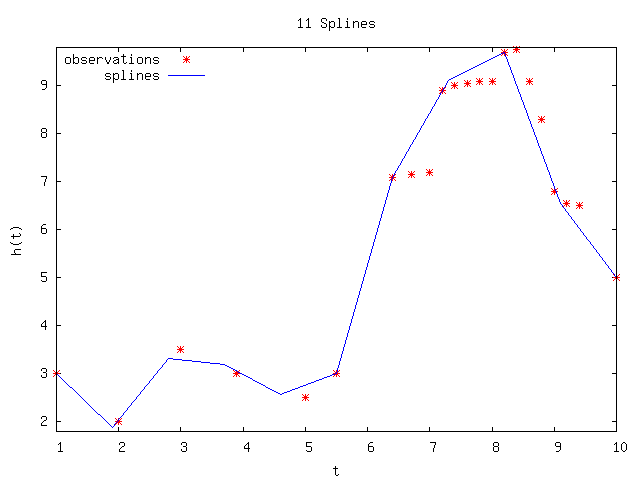
\includegraphics[height=35mm]{images/11splines}}}
    \end{picture}
\end{frame}
%%==================================================================Sb
\subsection{Detección de bordes}
%%==================================================================F
\begin{frame}
  \frametitle{Detección de bordes}
\begin{beamerboxesrounded}[shadow=true]{Definición: \emph{Borde}}
     \alt<1>{\alert<1>{NO} es un señor antipático $\Rightarrow$ \alert<1>{NO} 
        es tu jefe}{Es una fuerte variación en altura correspondiente a una 
        pequeña variación en planimetría}
    \end{beamerboxesrounded}

\only<2>{
  \begin{picture}(0,100)
    %\centering
    \begin{tikzpicture}[scale=0.7]
    \draw[thick] (-5,0) -- (2.5,0);
    \filldraw[black!20!white] (-2,0) -- (-2,2) -- (0,3) -- (2,2) -- (2,0) -- cycle;
    \draw (-2,0) -- (-2,2) -- (0,3) -- (2,2) -- (2,0) -- cycle;

    \coordinate[mark coordinate] (S) at (-2,0);
    \coordinate[mark coordinate] (B) at (-2,2);
    \node[anchor=south east] at (S){};
    \node[anchor=north west] at (B){};
    \node[anchor=west] at (-1,1){Objeto};
    \end{tikzpicture}
  \end{picture}
  \begin{picture}(0,100)
     \only<2>{\put(200,-5){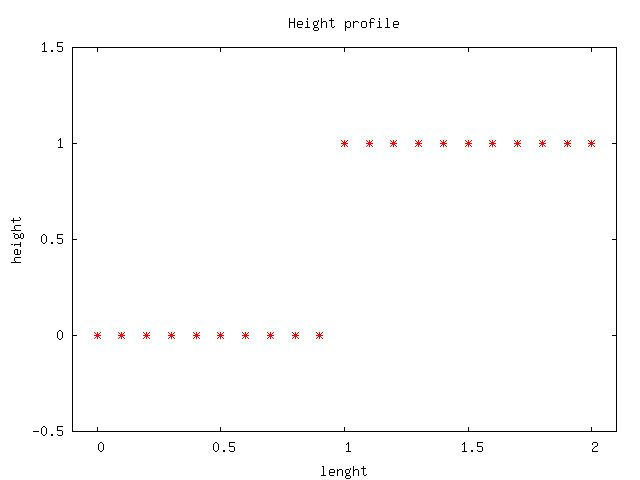
\includegraphics[height=30mm]{images/height_edge}}}
  \end{picture}
}
\begin{enumerate}
 \item<3-> El análisis de bordes no es fácil porque los puntos no están distribuidos regularmente
 \item<4-> Se pueden regularizar los puntos $\Rightarrow$ se rasteriza: 
    \begin{itemize}
        \item<4-> \alert<4>{mínimo} y \alert<4>{máximo}
	\item<5-> \alert<5>{Media}
	\item<6-> \alert<6>{Interpolación}
	\item<7-> \alert<7>{\emph{kriging}}...
    \end{itemize}
  \item<8-> \alert<8>{Pérdida de información} altimétrica
\end{enumerate}
\end{frame}
%%==================================================================F
\begin{frame}
  \frametitle{Cálculo de bordes}
\begin{enumerate}
  \item Se trabaja con una interpolación con spline bilineares que se ajuste 
    mucho a las observaciones (nuestros puntos)
  \item<2->{Para esta superficie se calcula:}
\begin{itemize}
 \item<2-> El \alert<2>{Gradiente} para cada punto: $G_m = \sqrt{G_x^2 + G_y^2} = \sqrt{\left( \dfrac{dz}{dx}\right)^2 + \left( \dfrac{dz}{dy}\right)^2}$
 \item<3-> La \alert<3>{dirección normal}: $\vartheta_P = \arctan\left(\dfrac{G_y}{G_x} \right)$
\end{itemize}
\end{enumerate}

  \uncover<4->{\alert<4>{Estos dos parámetros no son suficientes!!}}
\end{frame}
%%==================================================================F
\begin{frame}
  \frametitle{Valor gradiente}
  \begin{enumerate}[<+->]
   \item El gradiente tiene un valor muy alto en el borde de los objetos pero también el punto exterior más próximo
   \item Debido al ruido en las observaciones, el valor más alto del gradiente \alert<2>{puede ser el equivocado}
  \end{enumerate}
    \begin{picture}(0,110)
        \only<1>{\put(80,0){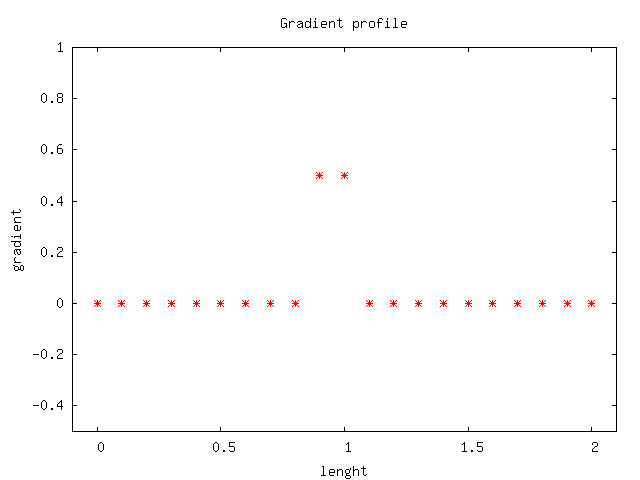
\includegraphics[height=40mm]{images/gradient_edge}}}
        \only<2>{\put(80,0){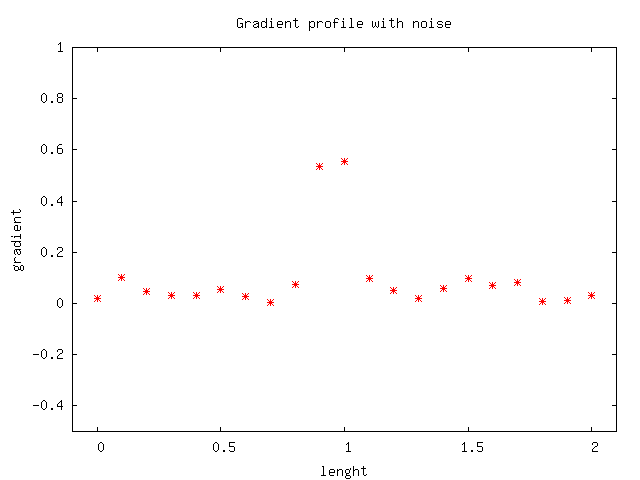
\includegraphics[height=40mm]{images/gradient_noise_edge}}}
    \end{picture}
\end{frame}
%%==================================================================F
\begin{frame}
  \frametitle{Cálculo de residuos}%
  \begin{enumerate}[<+->]%
   \item Se trabaja con una interpolación con spline bicúbicas con resolución muy baja 
       para obtener una \alert<1>{superficie muy lisa}%
   \item Se calcula el residuo entre la superficie y las observaciones%
   \item El punto con residuo positivo será nuestro \only<3>{\alert<3>{impertinente}}\only<4>{\alert<4>{borde} ;-) }%
  \end{enumerate}%
\uncover<3->{
  \begin{figure}[!b]
    \centering
    \begin{tikzpicture}[scale=0.85]
    %\includegraphics[height=50mm]{images/figure_6}
    \draw[thick] (-5,0) -- (3,0);
    \filldraw[black!20!white] (-2,0) -- (-2,2) -- (0,3) -- (2,2) -- (2,0) -- cycle;
    \draw (-2,0) -- (-2,2) -- (0,3)node[above]{Objeto} -- (2,2) -- (2,0) -- cycle;
    \draw[thick] (-4.5,0.3)node[above]{Interpolaci\'on} -- 
        (-3.5,0.3) .. controls (-1.5,.4) and (-1.5,2) .. (0,2);

    \coordinate[mark coordinate] (N) at (-2,0);
    \coordinate[mark coordinate] (P) at (-2,2);
    \node[anchor=south east] at (N){--};
    \node[anchor=north west] at (P){+};

    \node[anchor=west] at (-0.5,1){+ Borde};
    \node[anchor=west] at (-0.5,0.5){-- \  Terreno};
    \end{tikzpicture}
  \end{figure}
}
\end{frame}
%%==================================================================F
\begin{frame}
  \frametitle{Identificación final de bordes}%
  Para que un punto sea considerado como el borde de un objeto se debe cumplir:
  \begin{enumerate}[<+->]%
	\item El gradiente debe ser mayor que un cierto umbral dado por el usario
	\item Si el gradiente es grande pero \alert<2>{sin} llegar al umbral, además se debe verificar que:
	\begin{itemize}
	 \item El residuo es \alert<3>{positivo}
	 \item La dirección normal no se desvía mas de un valor dado.
	\end{itemize}
  \end{enumerate}
\end{frame}
%%==================================================================Sb
\subsection{Region Growing}
%%==================================================================F
\begin{frame}
  \frametitle{``Region Growing''}
\begin{beamerboxesrounded}[shadow=true]{Hipótesis}
El interior del objeto será siempre igual o más alto que los bordes (su altura media)
\end{beamerboxesrounded}

\begin{enumerate}
 \item El objetivo en este paso es reconocer el \alert{interior} de los objetos
 \item Para cada borde se construye un \alert{conj. convexo} y en su interior se ejecuta un algoritmo de \alert{\emph{region growing}} para verificar la hipótesis
\end{enumerate}
\end{frame}
%%==================================================================F
\begin{frame}
  \frametitle{Primera clasificación}
Los puntos viene clasificados por su posición con respecto al terreno: \pause
\begin{enumerate}
 \item \alert{Objeto}: Si están dentro del conj. convexo y su altura es mayor que la altura media del borde
 \item \alert{Terreno}: En cualquier otro caso.
\end{enumerate}

\pause
Y por el tipo de impulso:
\begin{enumerate}
 \item \alert{\'Unico impulso}: Si solo se ha recibido un eco de ese punto
 \item \alert{Doble impulso}: Si se han recibido más impulsos
\end{enumerate}
\end{frame}
%%==================================================================Sb
\subsection{Corrección}
%%==================================================================F
\mode<beamer>{
  \pgfdeclareimage[width=0.4\textwidth]{fumo}{images/fumo}
}
\begin{frame}
  \frametitle{Errores en la clasificación}
  \begin{columns}
    \begin{column}{0.5\textwidth}
     \begin{enumerate}
    	\item<1-> La hipótesis de las alturas falla
    	\item<2-> Se han identificado bordes pertenecientes al terreno pero no a objetos
     \end{enumerate}
    \end{column}
   \begin{column}{0.45\textwidth}
    %\only<1>{%
   \begin{center}
   	\begin{tikzpicture}
	\mode<beamer>{
    	  \pgftext[bottom,left,at={\pgfpointxy{2}{0}}]{\pgfuseimage{fumo}}
	}
	\mode<beamer:0>{
    	  \pgftext[bottom,left,at={\pgfpointxy{2}{0}}]{\pgfuseimage{fumog}}
	}
	\end{tikzpicture}
   \end{center}%
   %}
   \end{column}
  \end{columns}
\end{frame}
%%==================================================================F
\begin{frame}
  \frametitle{Corrección final}

Se utilizan los puntos \alert<1>{Terreno único impulso} para realizar una interpolación con splines bilineares y resolucion baja para obtener una superficie bastante lisa
\begin{enumerate}
 \item<2-> Si un punto terreno está lo suficientemente alejado de la superficie se reclasifica como \alert<2>{objeto}
 \item<3-> Si un punto objeto está lo suficientemente cercano a la superficie se reclasifica como \alert<3>{terreno}
\end{enumerate}
\end{frame}
%%==================================================================Sb
\subsection{Vegetación}
%%==================================================================F
\begin{frame}
 
\end{frame}
